\documentclass{article}

\usepackage{graphicx}
\usepackage{tikz}
\usepackage{tikzsymbols}
\usetikzlibrary{calc,patterns,shapes.geometric}
\pagestyle{empty}
\usepackage[margin=0pt]{geometry}
\geometry{papersize={14in,12in}}

\def\centerarc[#1](#2)(#3:#4:#5){\draw[#1] ($(#2)+({#5*cos(#3)},{#5*sin(#3)})$) arc (#3:#4:#5);}

\begin{document}
	\begin{figure}
		\centering
		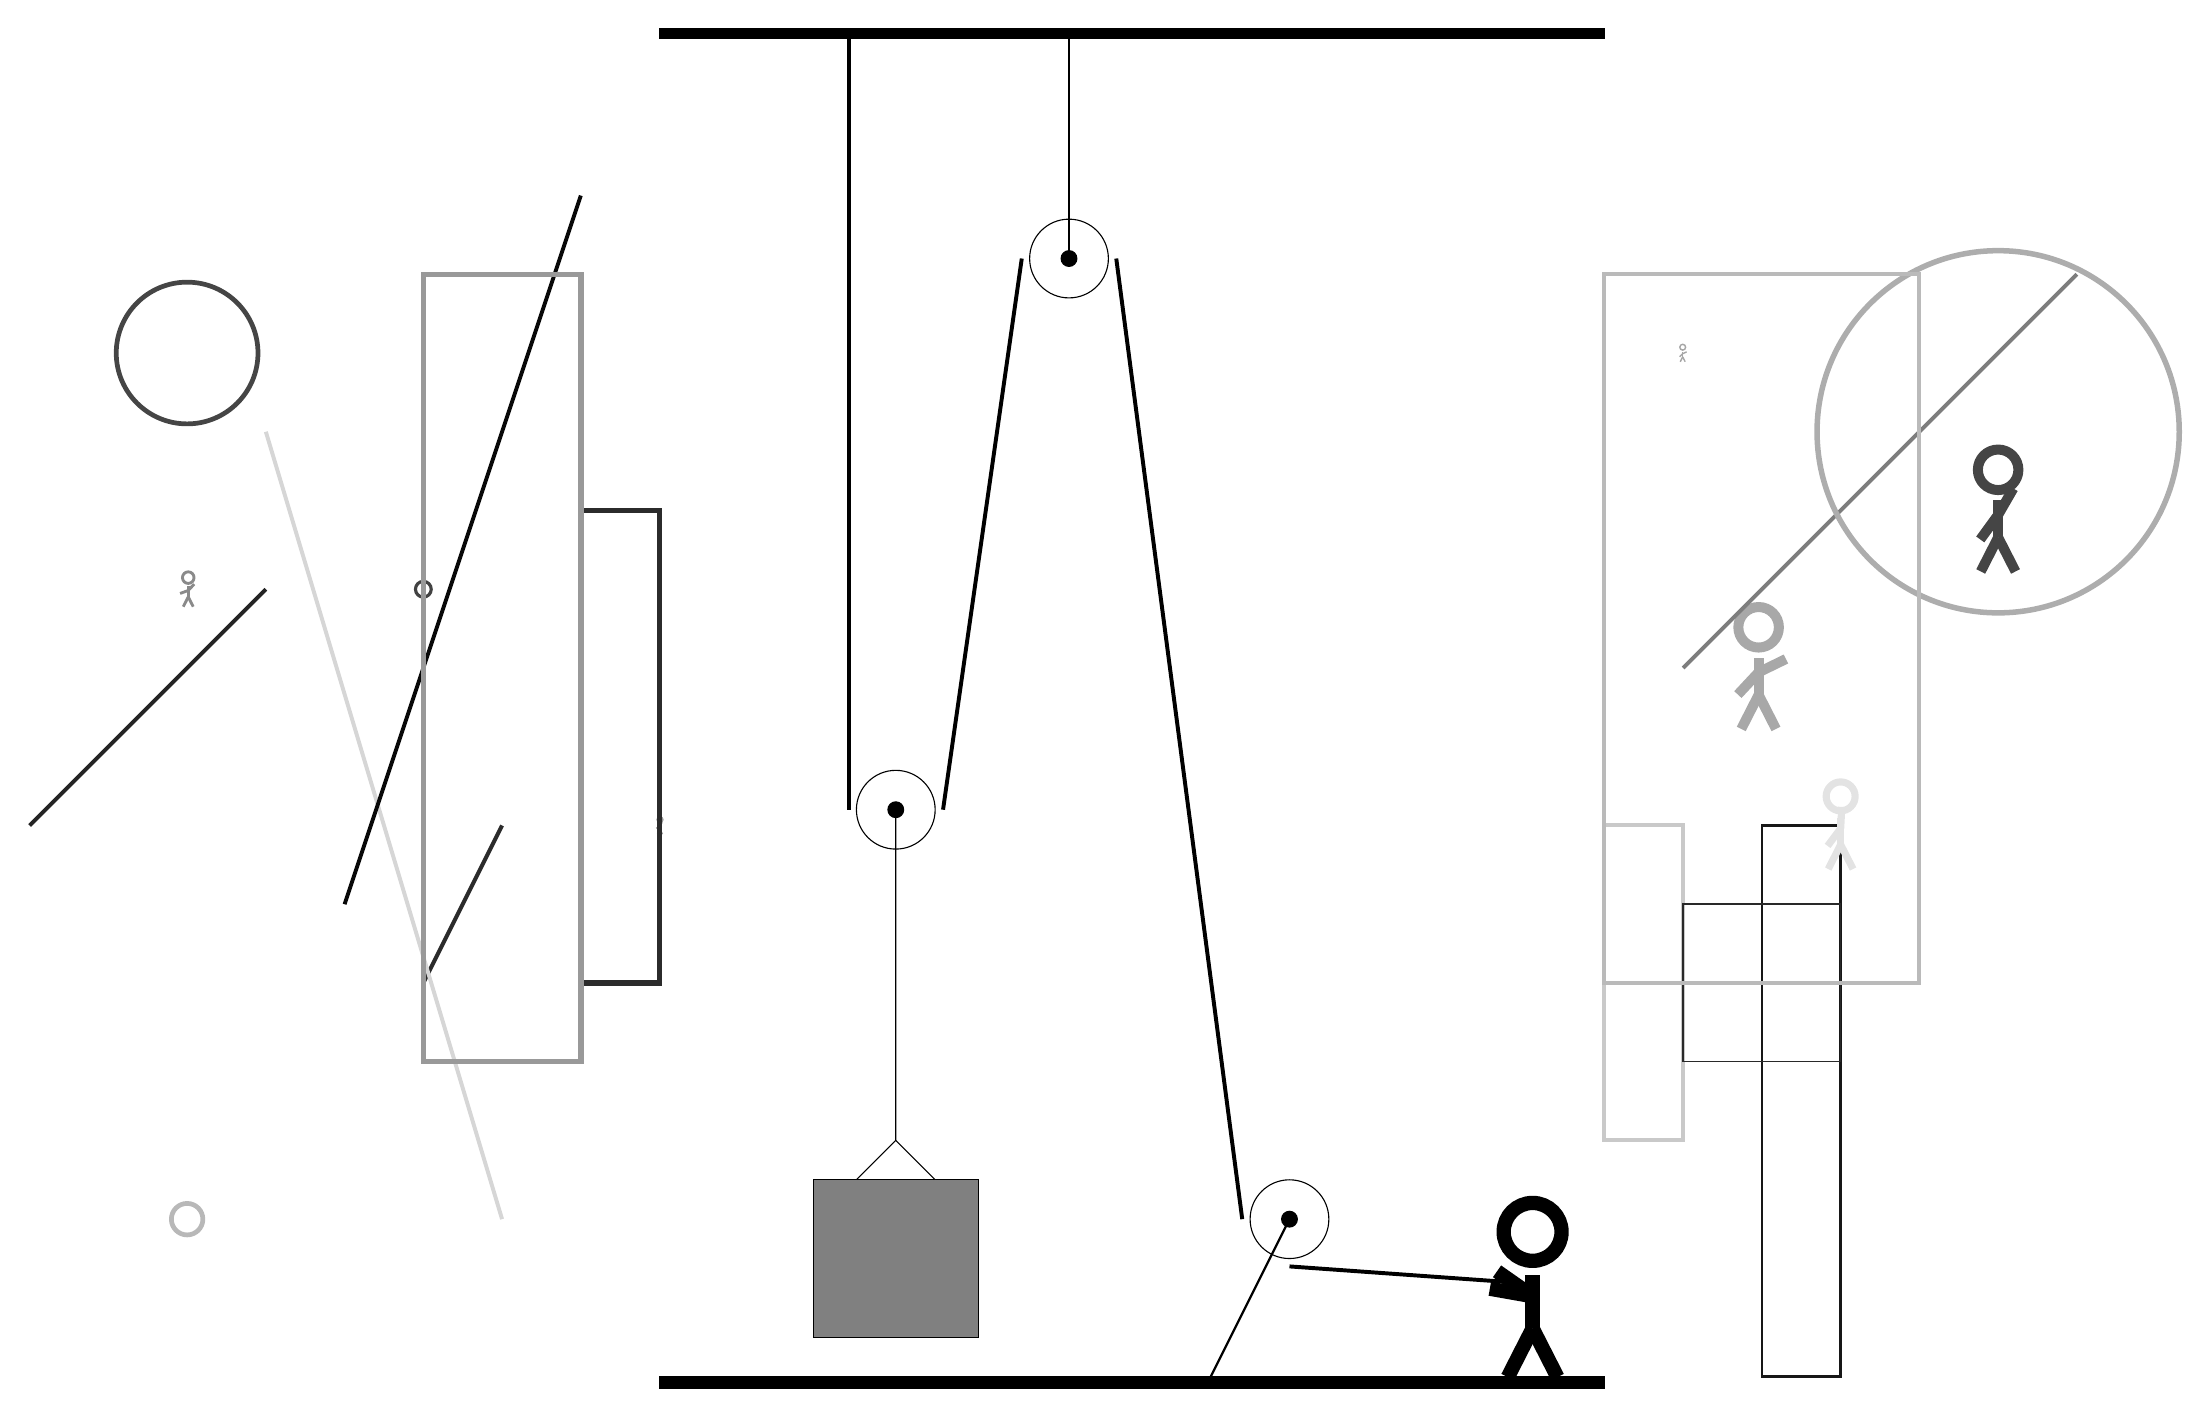
\begin{tikzpicture}
			%%%%% START %%%%%
			
			\draw[fill=black] (-2, 14) rectangle (10, 14.125);
			
			\draw[line width=0.4mm, color=black!32] (-2, 7) rectangle (-2, 2);
			
			\draw[line width=0.5mm, color=black!86](-7, 7) -- (-10, 4);
			\node[line width=0.2mm, color=black!34] at (12, 6) {\Strichmaxerl[7][47][26]};
			\node[line width=0.2mm, color=black!40] at (-2, 4) {\Strichmaxerl[1][31][60]};
			\draw [line width=0.6mm, color=black!73](-8, 10) circle (0.9);
			
			\draw[line width=0.3mm, color=black!91] (12, 4) rectangle (13, -3);
			
			\draw[line width=0.5mm, color=black!51](11, 6) -- (16, 11);
			
			\node[line width=0.5mm, color=black!11] at (13, 4) {\Strichmaxerl[5][53][87]};
			\node[line width=0.5mm, color=black!73] at (15, 8) {\Strichmaxerl[7][54][60]};
			\draw[line width=0.5mm, color=black!21] (10, 0) rectangle (11, 4);
			\draw[line width=0.5mm, color=black!83](-4, 4) -- (-5, 2);
			\draw[line width=0.2mm, color=black!84] (11, 3) rectangle (13, 1);
			\draw [line width=0.7mm, color=black!32](15, 9) circle (2.3);
			
			\draw[line width=0.5mm, color=black!27] (10, 11) rectangle (14, 2);
			\draw [line width=0.6mm, color=black!28](-8, -1) circle (0.2);
			\draw[line width=0.7mm, color=black!83] (-3, 2) rectangle (-2, 8);
			\node[line width=0.5mm, color=black!35] at (11, 10) {\Strichmaxerl[1][46][24]};
			\draw[line width=0.5mm, color=black!16](-7, 9) -- (-4, -1);
			\draw [line width=0.4mm, color=black!74](-5, 7) circle (0.1);
			
			\draw[line width=0.5mm, color=black!97](-6, 3) -- (-3, 12);
			\node[line width=0.6mm, color=black!46] at (-8, 7) {\Strichmaxerl[2][20][47]};
			\draw[line width=0.7mm, color=black!40] (-3, 1) rectangle (-5, 11);
			
			\draw (3.2, 11.2) circle (0.5);
			\draw[fill=black] (3.2, 11.2) circle (0.1);
			\draw[thick] (3.2, 11.2) -- (3.2, 14);
			
			\draw (6, -1) circle (0.5);
			\draw[fill=black] (6, -1) circle (0.1);
			\draw[thick] (6, -1) -- (5, -3);
			
			\draw (1, 4.2) circle (0.5);
			\draw[fill=black] (1, 4.2) circle (0.1);
			
			\draw (1, 4.2) -- (1, 0) -- (0.5, -0.5);
			\draw (1, 0) -- (1.5, -0.5);
			\draw[fill=black!50] (-0.05, -0.5) rectangle (2.05, -2.5);
			
			\draw[line width=0.5mm] (0.4, 14) -- (0.4, 4.2);
			\centerarc[line width=0.5mm](1, 4.2)(180:360:0.6);
			\draw[line width=0.5mm](1.6, 4.2) -- (2.6, 11.2);
			\centerarc[line width=0.5mm](3.2, 11.2)(0:180:0.6);
			\draw[line width=0.5mm](3.8, 11.2) -- (5.4, -1);
			\centerarc[line width=0.5mm](6, -1)(180:270:0.6);
			\draw[line width=0.5mm](6, -1.6) -- (8.8, -1.8);
			
			\node at (9, -1.9) {\Strichmaxerl[10][-35][170]};
			
			\draw[fill=black] (-2, -3) rectangle (10, -3.15);
			
			%%%%% END %%%%%
		\end{tikzpicture}
	\end{figure}	
\end{document}